% !TEX TS-program = xelatex
% !TEX encoding = UTF-8 Unicode
%
\documentclass{beamer}
%\setbeamertemplate{items}[ball] 
%\DeclareMathOperator*{\argmax}{arg\,max}
\usecolortheme{whale}
\useinnertheme[shadow]{rounded}
\usenavigationsymbolstemplate{}
\usepackage[subsection=false,headline=empty,footline=outlineauthortitle]{beamerouterthememiniframesbottom}
%\usepackage{beamerthemesplit}
\usepackage{tikz}
\usepackage{pgfplots}
\usetikzlibrary{arrows,automata,positioning,shapes,shapes.geometric,fit,tikzmark,calc}
\usefonttheme[onlymath]{serif}
\usepackage{bm}
\usepackage{enumitem}

\usepackage{textcomp}
% Set up citation style
\usepackage{natbib}
\usepackage{bibentry}
\bibpunct{(}{)}{;}{a}{,}{,}
\newcommand{\newcite}[1]{\citet{#1}}
\renewcommand{\cite}[1]{\citep{#1}}

%\setbeamercovered{transparent}

% Specify that no bibliography should be printed
\bibliographystyle{plainnat}


\setbeamertemplate{footline}[frame number]{}

%gets rid of bottom navigation symbols
\setbeamertemplate{navigation symbols}{}

%gets rid of footer
%will override 'frame number' instruction above
%comment out to revert to previous/default definitions
\setbeamertemplate{footline}{}

\usepackage{pgfpages}
\usepackage{graphicx}
\usepackage{enumitem}
\setlist[itemize,1]{label={\fontfamily{cmr}\fontencoding{T1}\selectfont\textbullet}}

\usepackage{mathtools}

\newcommand\defeq{\stackrel{\mathclap{\normalfont\mbox{\tiny def}}}{=}}
\newcommand{\Lim}[1]{\raisebox{0.5ex}{\scalebox{0.8}{$\displaystyle \lim_{#1}\;$}}}


\usecolortheme{whale}
\useinnertheme[shadow]{rounded}
\usenavigationsymbolstemplate{}
\usepackage[subsection=false,headline=empty,footline=outlineauthortitle]{beamerouterthememiniframesbottom}
\setbeamertemplate{footline}[frame number]{}

%gets rid of bottom navigation symbols
\setbeamertemplate{navigation symbols}{}

%gets rid of footer
%will override 'frame number' instruction above
%comment out to revert to previous/default definitions
\setbeamertemplate{footline}{}

\usepackage{fontspec} % Used by polyglossia
%\defaultfontfeatures{Ligatures=TeX}

%\usepackage{polyglossia}
%\setmainlanguage{english}
%\setotherlanguages{russian,ukrainian}
\setsansfont{Doulos SIL}
%\setsansfont{Noto Sans UI}
%\newfontfamily\ipafont{Doulos SIL}
%\newfontfamily\hawaiifont{Doulos SIL}
%\usepackage{pgfplots}

%\usepackage{ dsfont }
%\setbeamertemplate{note page}[plain]
%\setbeameroption{show notes on second screen=right}
%\usepackage{minted}
\title{2nd Workshop on Computational Methods for Endangered Languages (ComputEL-2)}
%\input{author}
%\input{institution}
\institute{University of Hawaiʻi at Mānoa}

\date{6-7 March 2017}

\begin{document}

\frame{
\titlepage
}

\frame{\frametitle{Speed dating: CS + Ling}
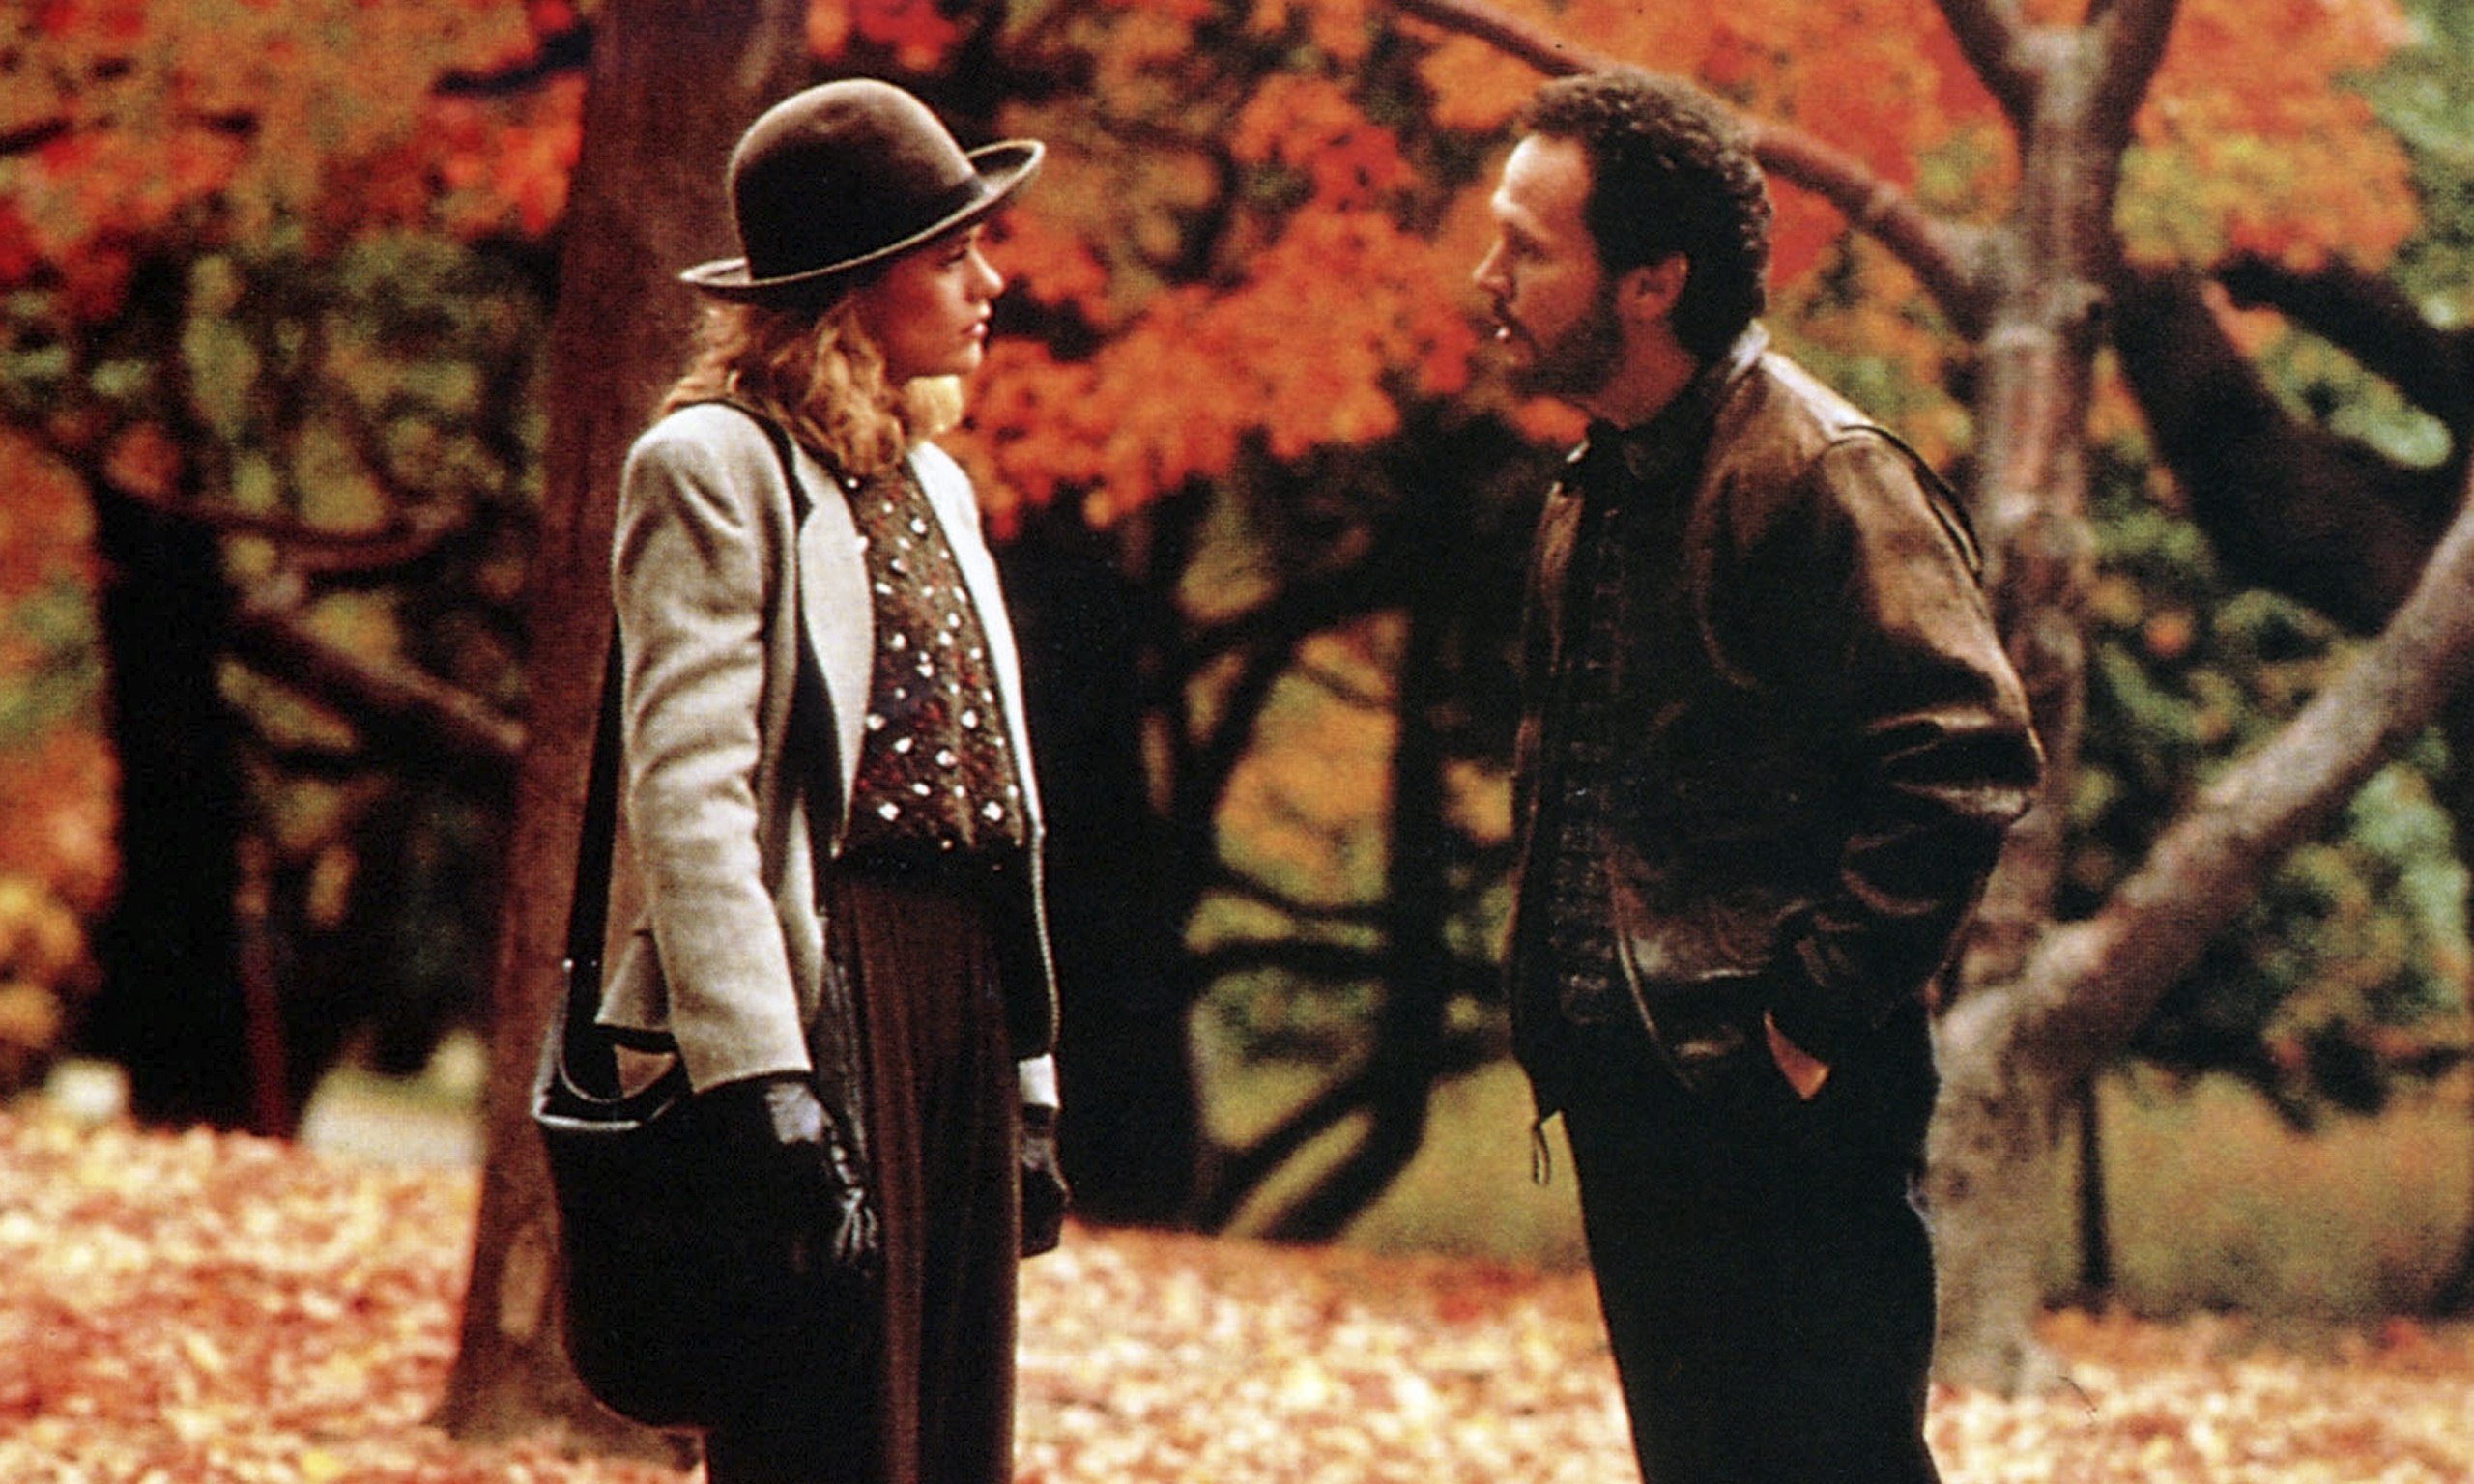
\includegraphics[width=1.0\textwidth]{harrysally}
}

\frame{\frametitle{Who you gonna call?}
\begin{center}
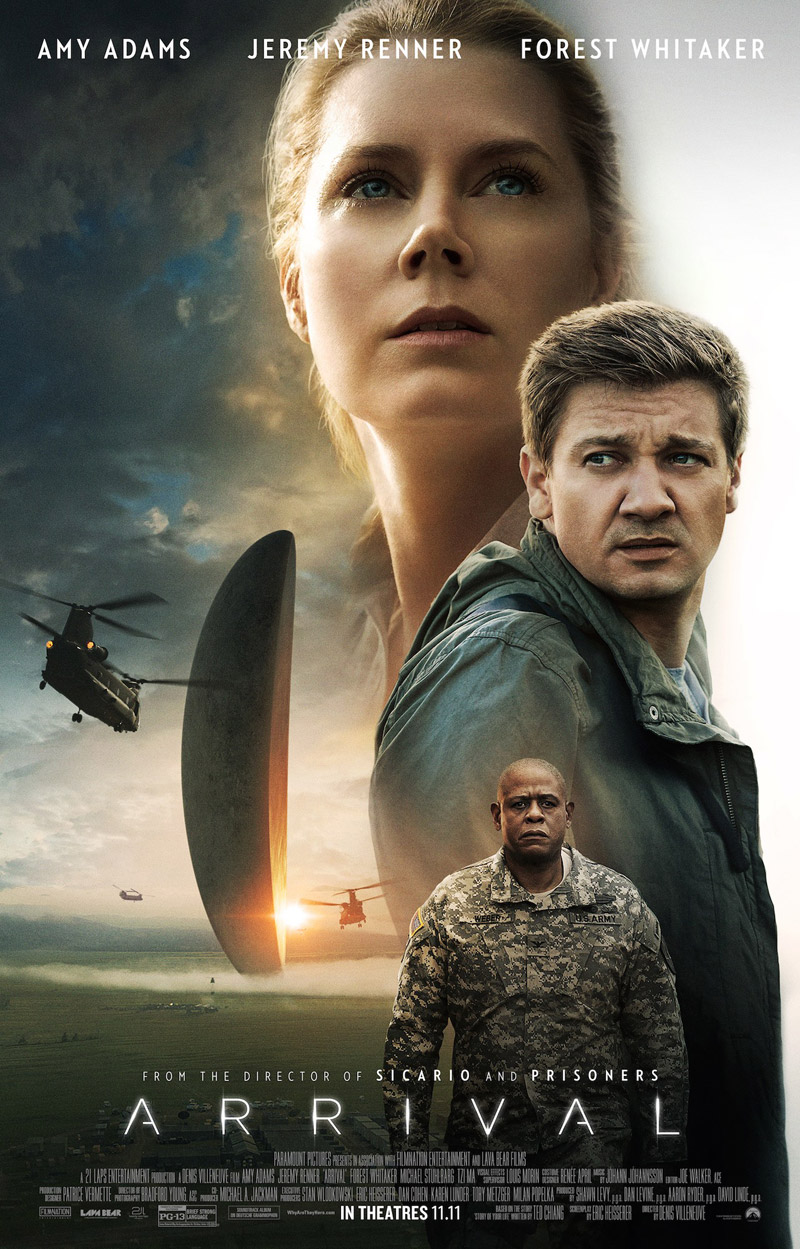
\includegraphics[width=0.48\textwidth]{arrivalposter}
\end{center}
}


\frame{\frametitle{Sponsors}

\begin{itemize}
\item U.S. National Science Foundation \\ Documenting Endangered Languages program \\ \ 
%
\item Social Sciences and Humanities Research Council of Canada \\ \ 
%
\item Sponsoring agencies of various participating researchers \\ \ 
%
\item Substantial organizational support from the ICLDC organizers and the University of Hawaiʻi at Mānoa
%
\end{itemize}

}

\frame{\frametitle{Organizing Committee}

\begin{itemize}
\item Antti Arppe (University of Alberta) \\ \
\item Jeff Good (University at Buffalo) \\ \
\item Mans Hulden (University Colorado at Boulder) \\ \ 
\item Jordan Lachler (University of Alberta) \\ \
\item Alexis Palmer (University of North Texas) \\ \ 
\item Lane Schwartz (University of Illinois at Urbana-Champaign)
%
\end{itemize}

}
 
 
\frame{\frametitle{Association for Computational Linguistics}

\begin{itemize}
%
\item Association for Computational Linguistics \\ ACL 2017 in Vancouver (July 30 -- Aug 4) \\ \ 
%
\item Regional ACL conferences in North America (NAACL), Europe (EACL), and Asia-Pacific (IJCNLP); in addition \\ Empirical Methods in Natural Language Processing (EMNLP) \\ \ 
%
\item Computational Linguistics (CL) and \\ Transactions of the ACL (TACL) journals \\ \ 
%
\item 19 ACL Special Interest Groups \\ (including phonology, morphology, and parsing): \\ \url{https://www.aclweb.org/portal/sigs} \\ \ 
%
\end{itemize}

}



\frame{\frametitle{URLs}

\begin{itemize}
%
\item This workshop (including schedule): \\ \url{http://altlab.artsrn.ualberta.ca/computel-2}  \\ \ \\ \
%
\item Proceedings: \\ \url{http://aclweb.org/anthology}
%
\end{itemize}

}

\end{document}
